
\documentclass[compress]{beamer}

\mode<presentation> {

    \usetheme{default}
    \useoutertheme{seb}
    \useinnertheme{seb}
% \usefonttheme{seb}
%\useoutertheme[subsection=false]{smoothbars} 


    \setbeamertemplate{navigation symbols}{} 
}
\usepackage{graphicx} 
\usepackage{booktabs}
\usepackage{amssymb} 

%----------------------------------------------------------------------------------------
%	TITLE PAGE
%----------------------------------------------------------------------------------------

\title{Introduction to Markov Chain Monte Carlo}

% \author{Helen Johnson}
\date{}

\begin{document}

    \begin{frame}
        \titlepage
    \end{frame}

    \section{Rejection sampling}
    \label{sec-5}
    \begin{frame}[label=sec-5-1]{Recap. on Bayesian inference}
        Last time we saw that the \alert{posterior distribution} of $\theta$, given observed data is

        $$ p(\theta | \text{data}) \propto p(\text{data}|\theta) p(\theta)$$\\~\\

        Our aim is to draw samples from this distribution.
    \end{frame}

    \begin{frame}[label=sec-5-2]{Rejection sampling}
        \begin{columns}[c] 
        \column{.5\textwidth} 
        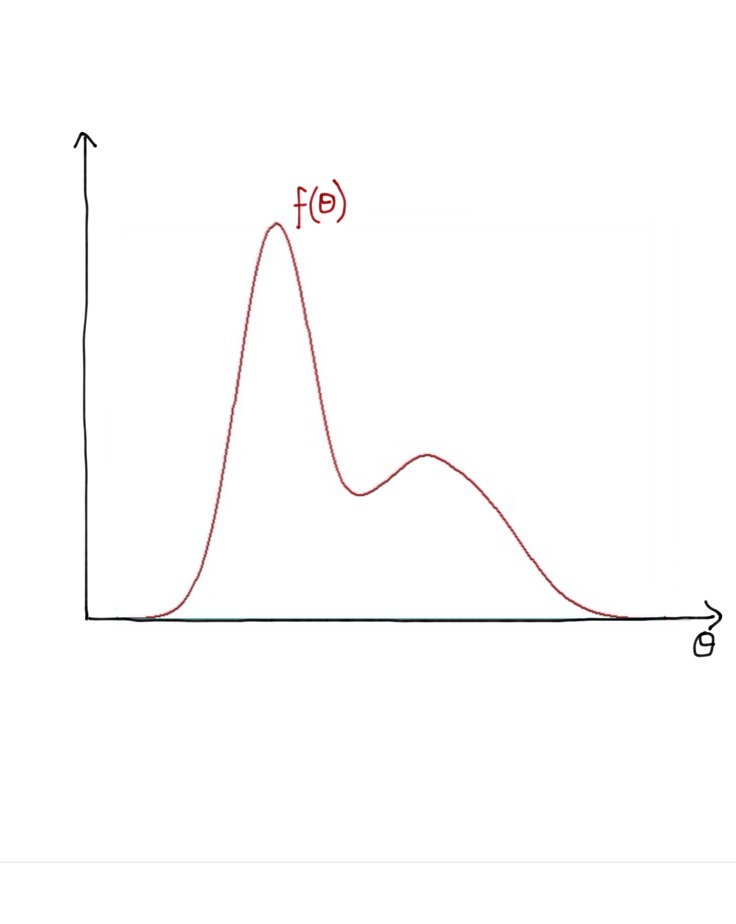
\includegraphics[width=1\linewidth]{RS1}

        \column{.6\textwidth}
        \begin{itemize}
            \item Consider a distribution $f(\theta)$,which we can evaluate for any $\theta$\\~\\
            \item How do we draw samples?
        \end{itemize}
    \end{columns}
\end{frame}

\begin{frame}[label=sec-5-3]{Rejection sampling}
    \begin{columns}[c] 
    \column{.5\textwidth} 
    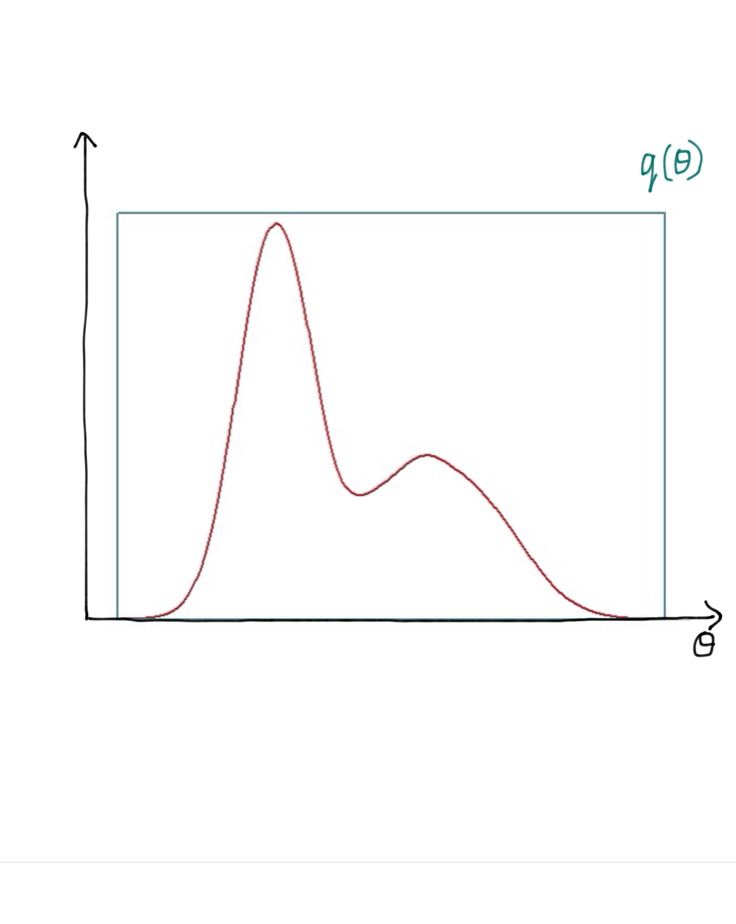
\includegraphics[width=1\linewidth]{RS2}

    \column{.6\textwidth}
    Rejection sampling uses a \alert{proposal distribution $q(\theta)$} which:
    \begin{itemize}
        \item is simple to evaluate
        \item is easy to sample from
        \item one can find $M>1$ such that $f(\theta) < M q(\theta)$ for all $\theta$
    \end{itemize}
\end{columns}
\end{frame}

\begin{frame}[label=sec-5-4]{Rejection sampling}
    \begin{columns}[c] 
    \column{.5\textwidth} 
    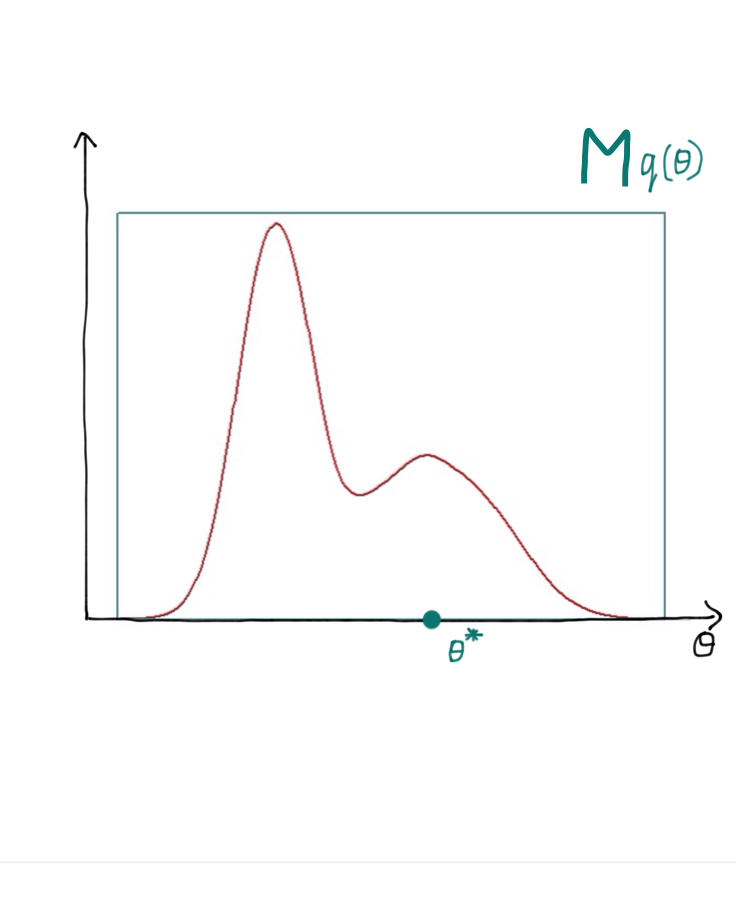
\includegraphics[width=1\linewidth]{RS3}

    \column{.6\textwidth}
    The algorithm proceeds as follows:\\
    \begin{enumerate}
        \item Sample $\theta^*$ from $q(\theta)$ \\~\\
        \textcolor{white}{
            \item[\color{white}] Draw $u \sim Uniform[0, Mq(\theta^*)]$ \\~\\
            \item[\color{white}] Evaluate $f(\theta^*)$ \\~\\
            \item[\color{white}] If $f(\theta^*) > u$ accept, else reject \\~\\
            \item[\color{white}] Repeat steps 1-4
        }
    \end{enumerate}
\end{columns}
\end{frame}

\begin{frame}[label=sec-5-5]{Rejection sampling}
    \begin{columns}[c] 
    \column{.5\textwidth} 
    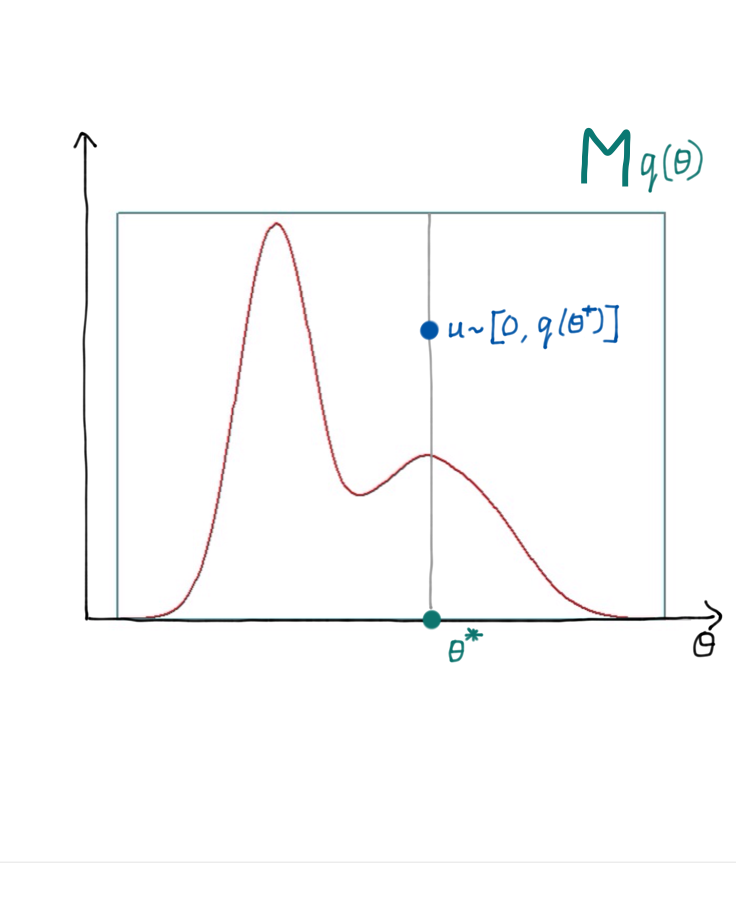
\includegraphics[width=1\linewidth]{RS4}

    \column{.6\textwidth}
    The algorithm proceeds as follows:\\
    \begin{enumerate}
        \item Sample $\theta^*$ from $q(\theta)$ \\~\\
        \item Draw $u \sim Uniform[0, Mq(\theta^*)]$ \\~\\
        \textcolor{white}{
            \item[\color{white}] Evaluate $f(\theta^*)$ \\~\\
            \item[\color{white}]If $f(\theta^*) > u$ accept, else reject \\~\\
            \item[\color{white}] Repeat steps 1-4
        }
    \end{enumerate}
\end{columns}
\end{frame}

\begin{frame}[label=sec-5-6]{Rejection sampling}
    \begin{columns}[c] 
    \column{.5\textwidth} 
    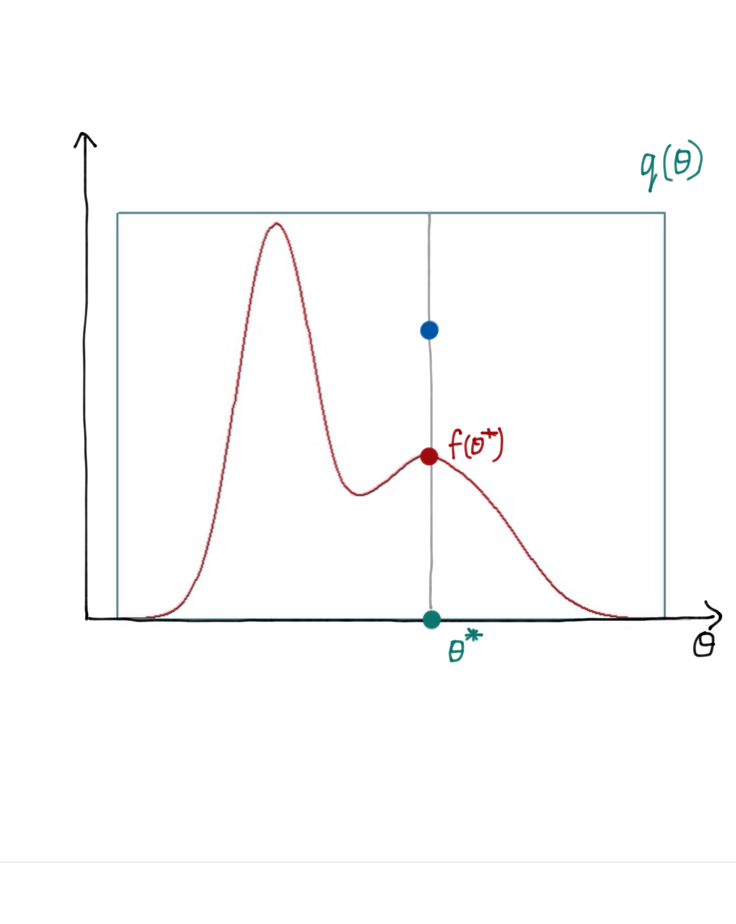
\includegraphics[width=1\linewidth]{RS5.png}

    \column{.6\textwidth}
    The algorithm proceeds as follows:\\
    \begin{enumerate}
        \item Sample $\theta^*$ from $q(\theta)$ \\~\\
        \item Draw $u \sim Uniform[0, Mq(\theta^*)]$ \\~\\
        \item Evaluate $f(\theta^*)$ \\~\\
        \textcolor{white}{
            \item[\color{white}] If $f(\theta^*) > u$ accept, else reject \\~\\
            \item[\color{white}] Repeat steps 1-4
        }
    \end{enumerate}
\end{columns}
\end{frame}

\begin{frame}[label=sec-5-7]{Rejection sampling}
    \begin{columns}[c] 
    \column{.5\textwidth} 
    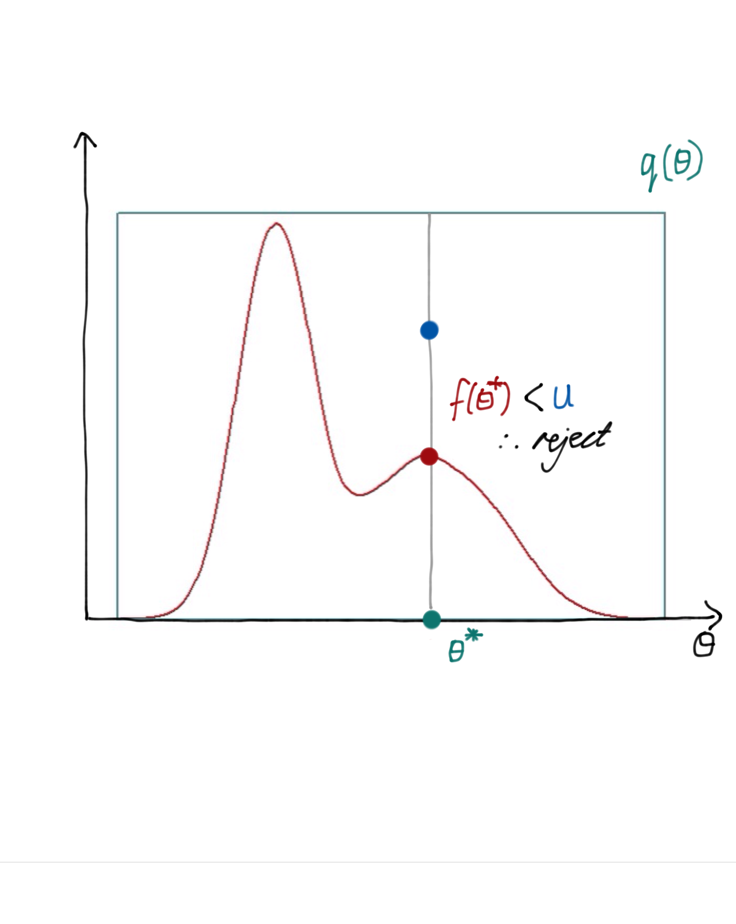
\includegraphics[width=1\linewidth]{RS6.png}

    \column{.6\textwidth}
    The algorithm proceeds as follows:\\
    \begin{enumerate}
        \item Sample $\theta^*$ from $q(\theta)$ \\~\\
        \item Draw $u \sim Uniform[0, Mq(\theta^*)]$ \\~\\
        \item Evaluate $f(\theta^*)$ \\~\\
        \item If $f(\theta^*) > u$ accept, else reject \\~\\
        \textcolor{white}{
            \item[\color{white}] Repeat steps 1-4
        }
    \end{enumerate}
\end{columns}
\end{frame}

\begin{frame}[label=sec-5-8]{Rejection sampling}
    \begin{columns}[c] 
    \column{.5\textwidth} 
    \only<1>{\href{RS7.png}{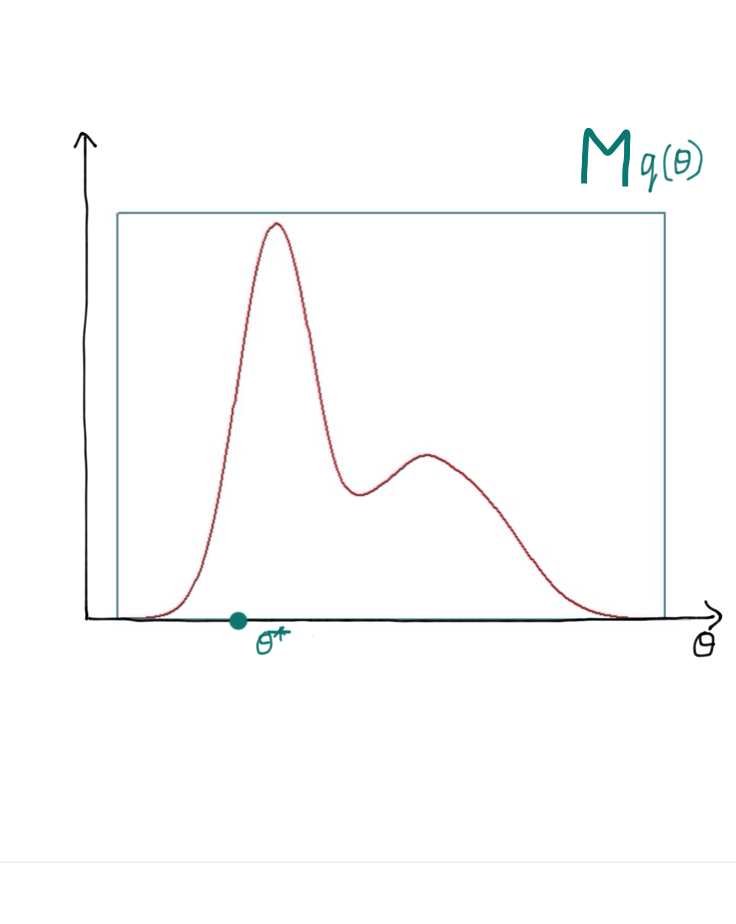
\includegraphics[width=1\linewidth]{RS7.png}}}
    \only<2>{\href{RS8.png}{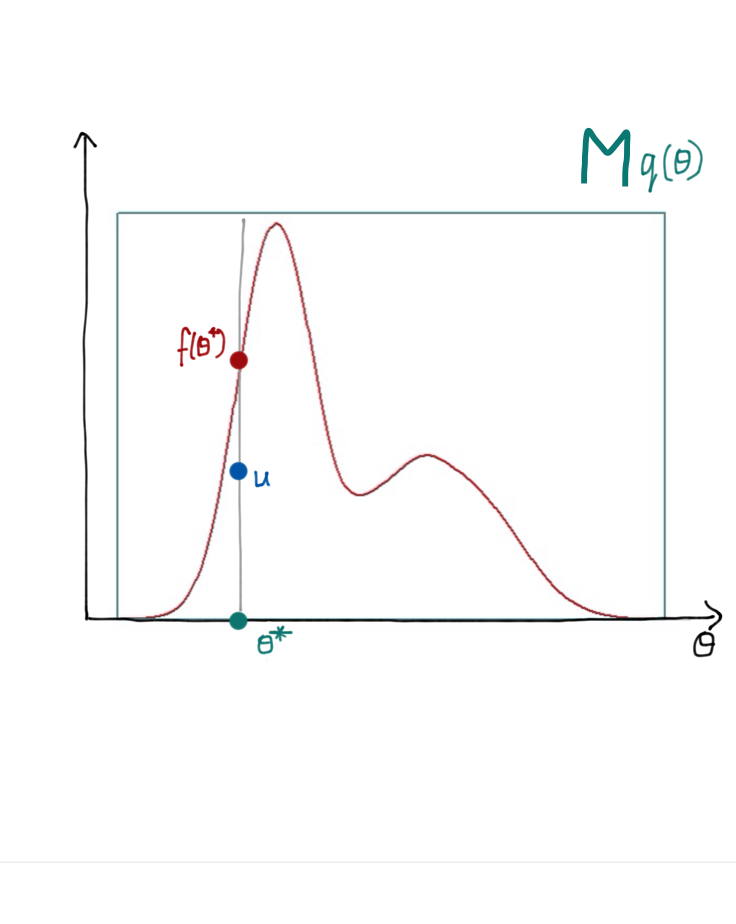
\includegraphics[width=1\linewidth]{RS8.png}}}
    \only<3>{\href{RS9.png}{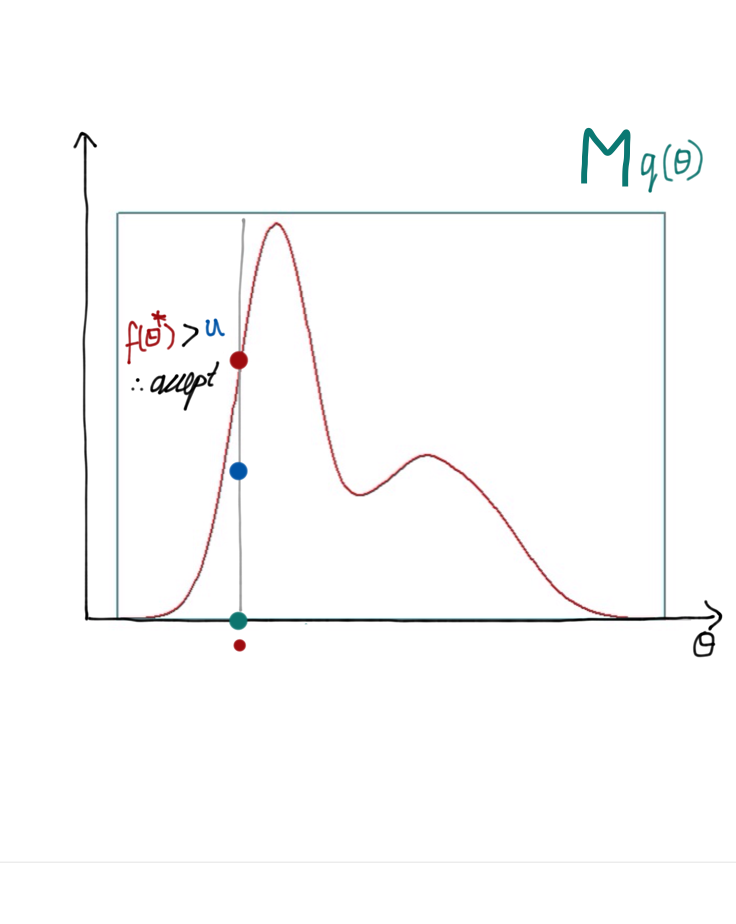
\includegraphics[width=1\linewidth]{RS9.png}}}
    \only<4>{\href{RS10.png}{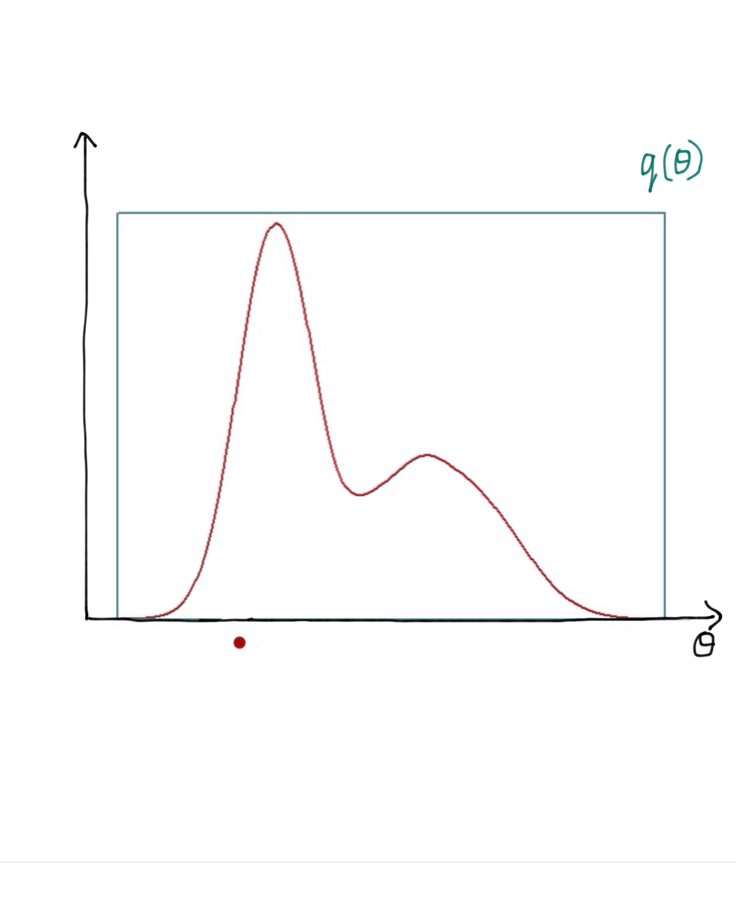
\includegraphics[width=1\linewidth]{RS10.png}}}
    \only<5>{\href{RS11.png}{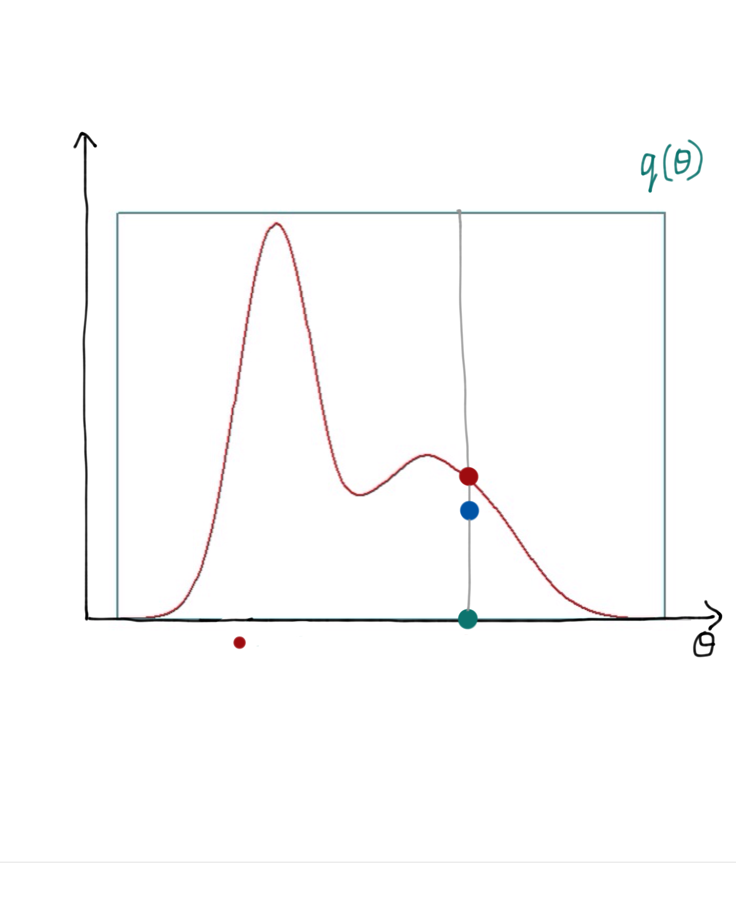
\includegraphics[width=1\linewidth]{RS11.png}}}
    \only<6>{\href{RS12.png}{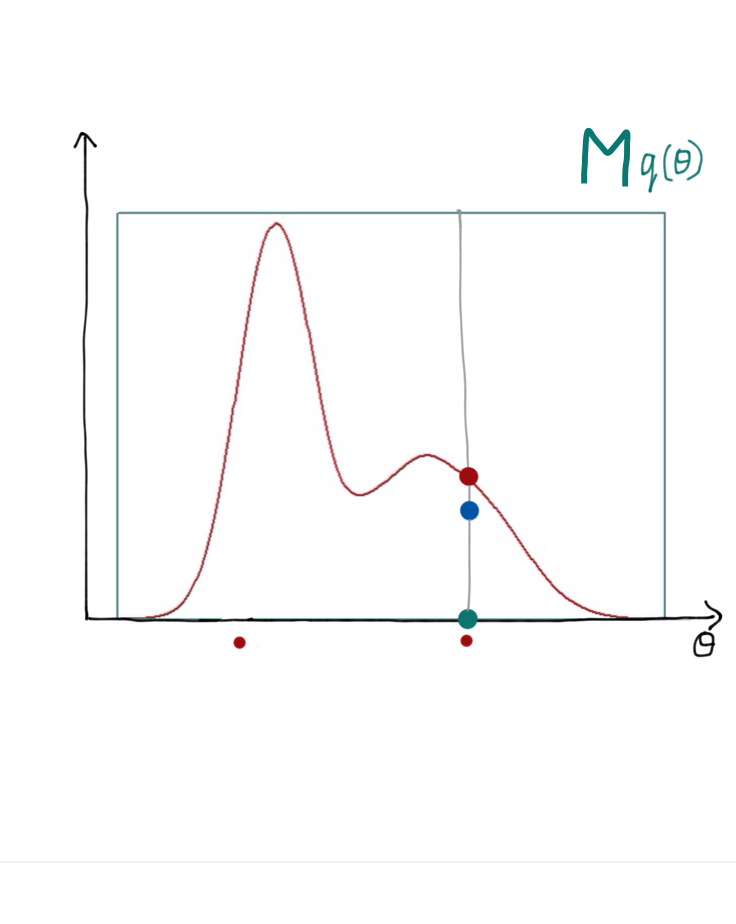
\includegraphics[width=1\linewidth]{RS12.png}}}
    \only<7>{\href{RS13.png}{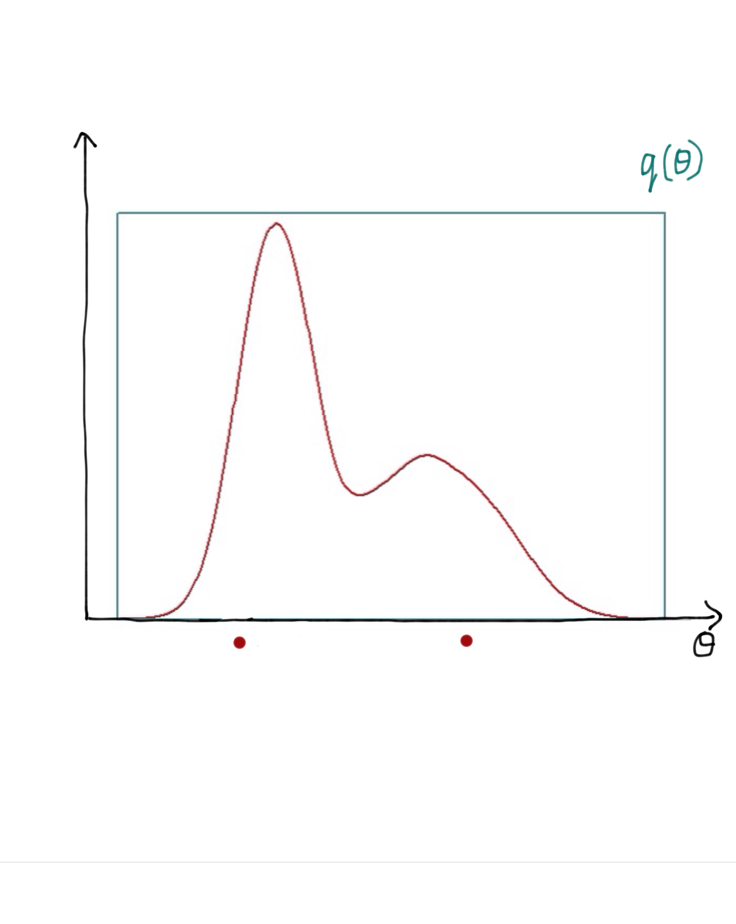
\includegraphics[width=1\linewidth]{RS13.png}}}
    \only<8>{\href{RS14.png}{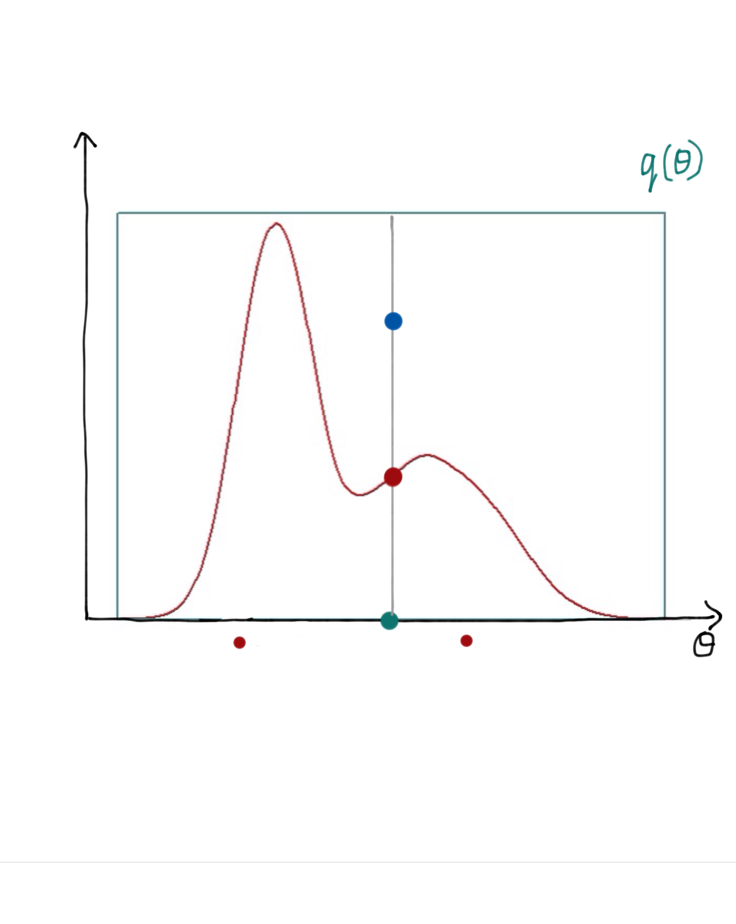
\includegraphics[width=1\linewidth]{RS14.png}}}
    \only<9>{\href{RS15.png}{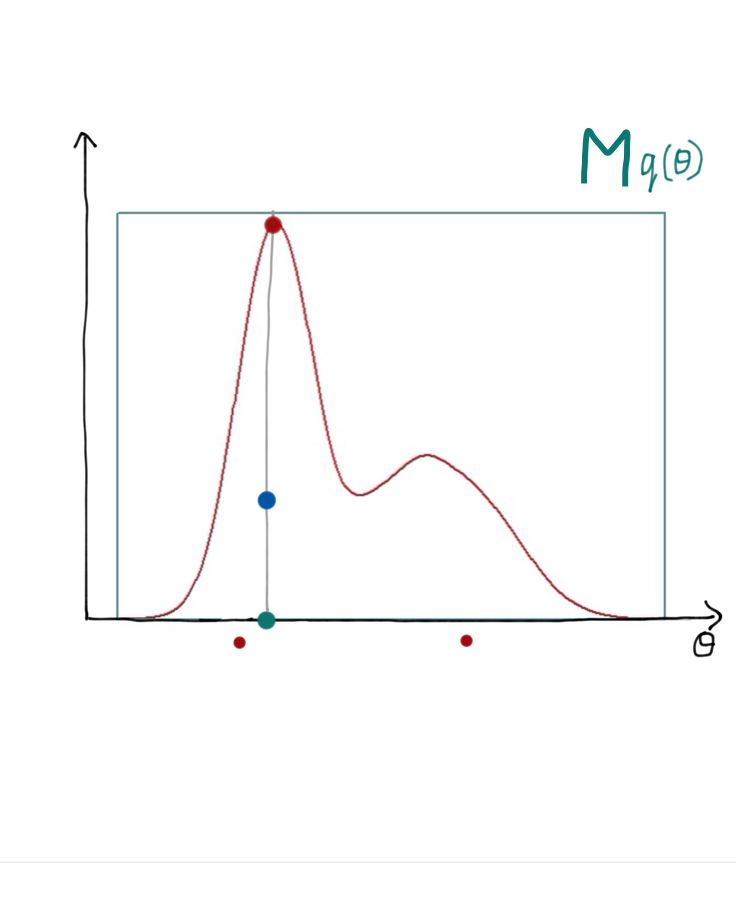
\includegraphics[width=1\linewidth]{RS15.png}}}
    \only<10>{\href{RS16.png}{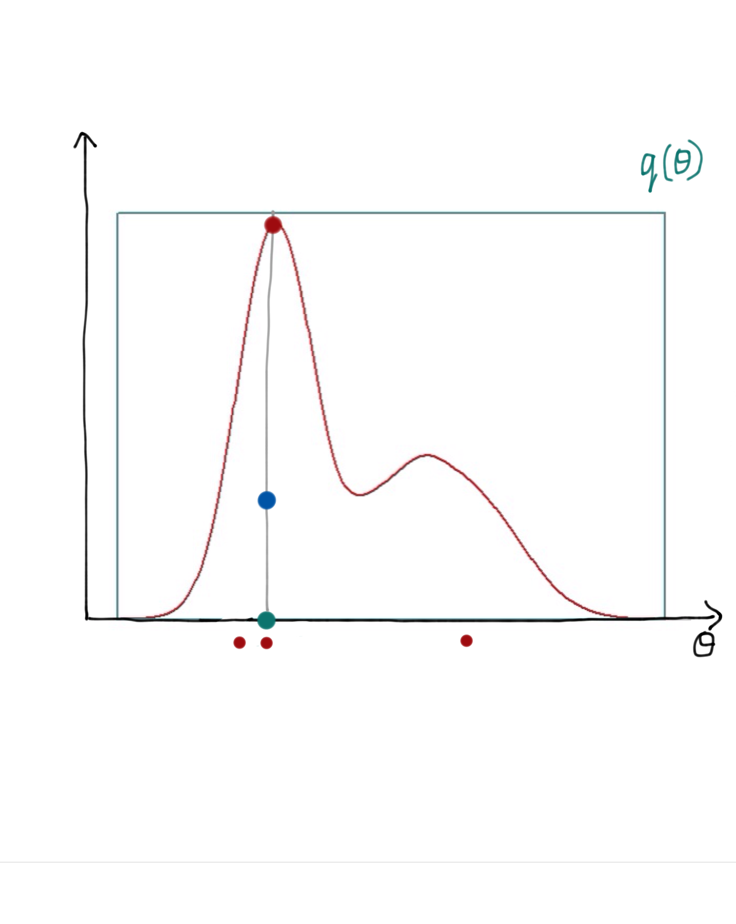
\includegraphics[width=1\linewidth]{RS16.png}}}
    \only<11>{\href{RS17.png}{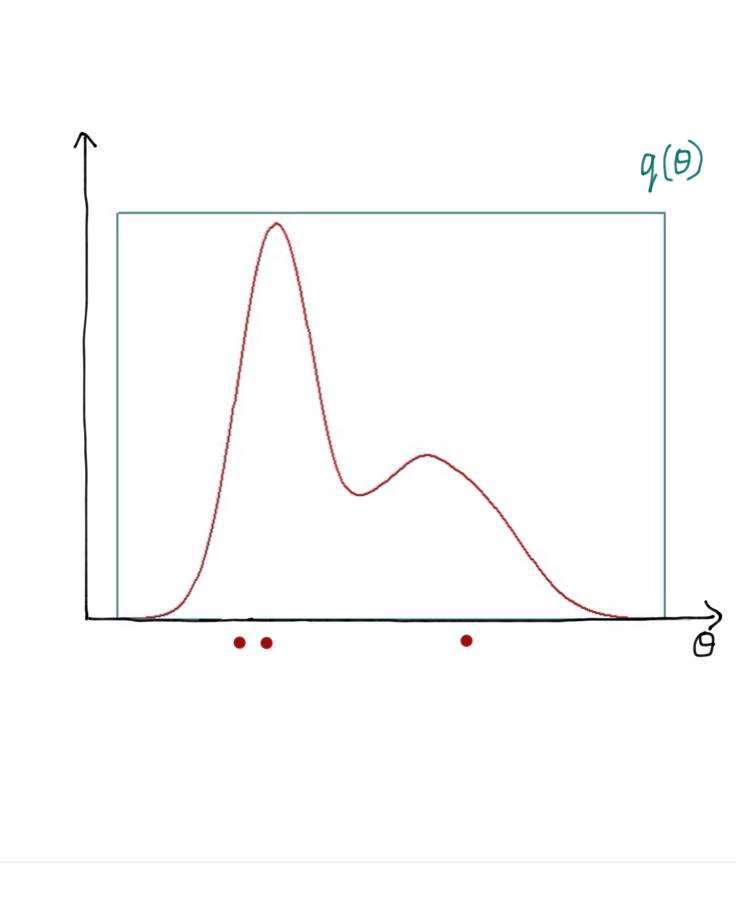
\includegraphics[width=1\linewidth]{RS17.png}}}
    \only<12>{\href{RS18.png}{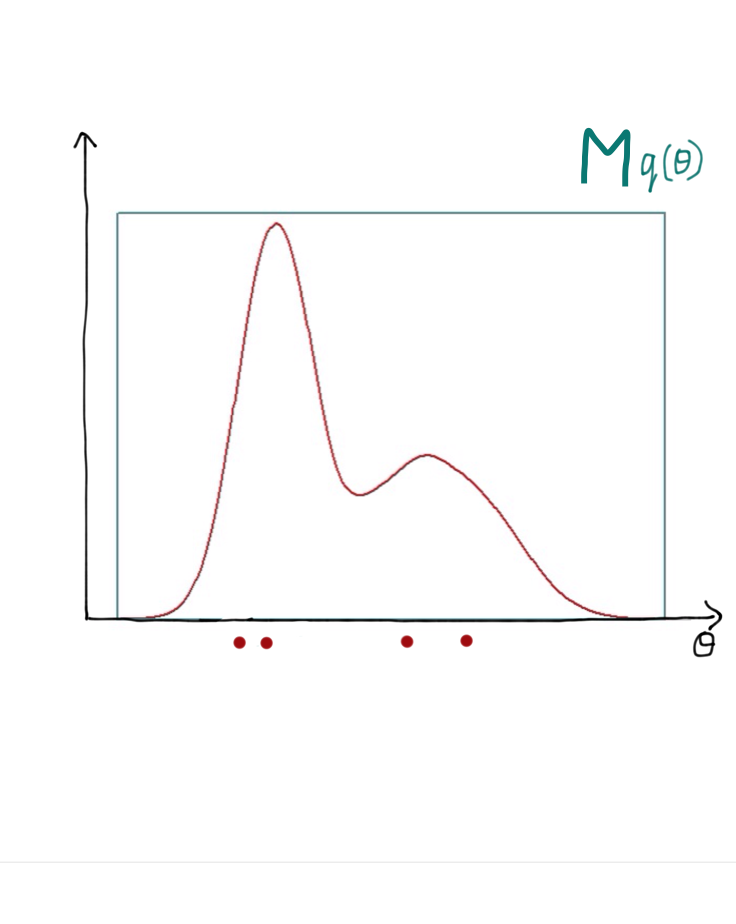
\includegraphics[width=1\linewidth]{RS18.png}}}
    \only<13>{\href{RS19.png}{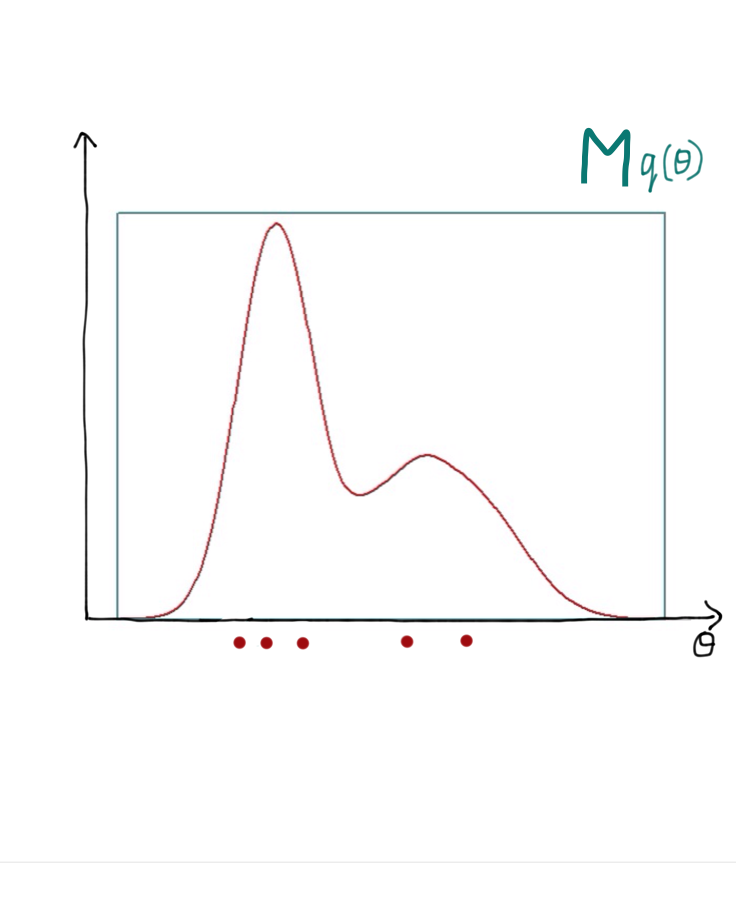
\includegraphics[width=1\linewidth]{RS19.png}}}
    \only<14>{\href{RS20.png}{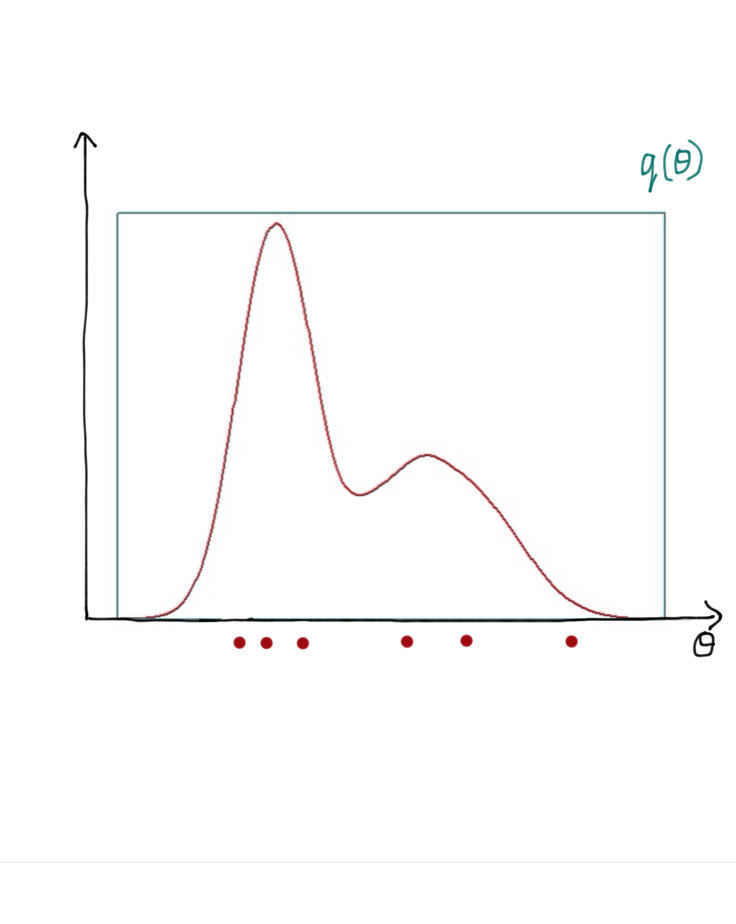
\includegraphics[width=1\linewidth]{RS20.png}}}
    \only<15>{\href{RS21.png}{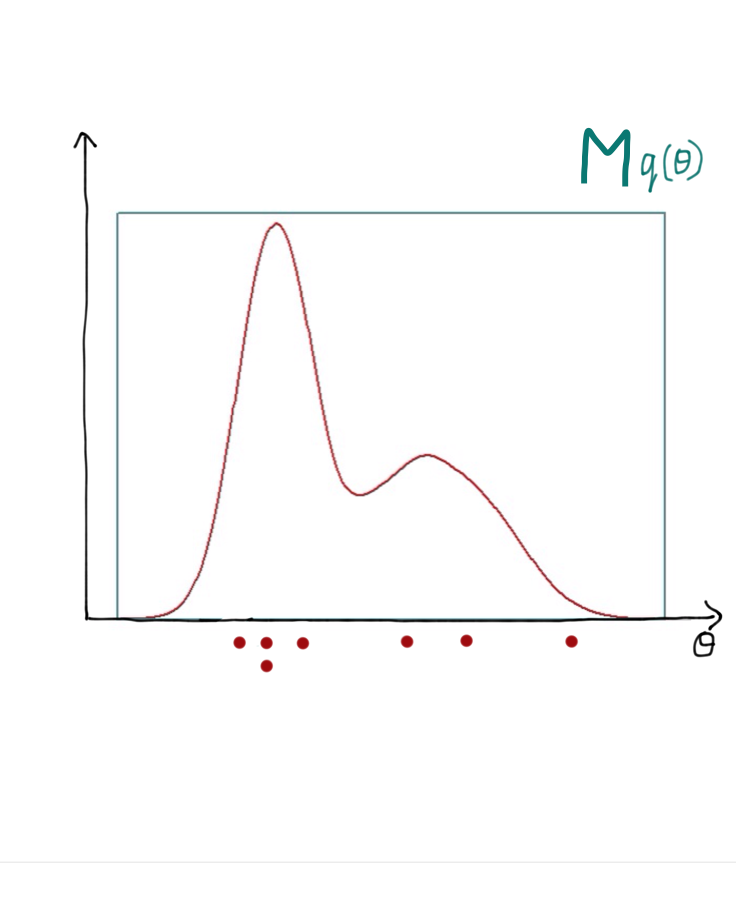
\includegraphics[width=1\linewidth]{RS21.png}}}
    \only<16>{\href{RS22.png}{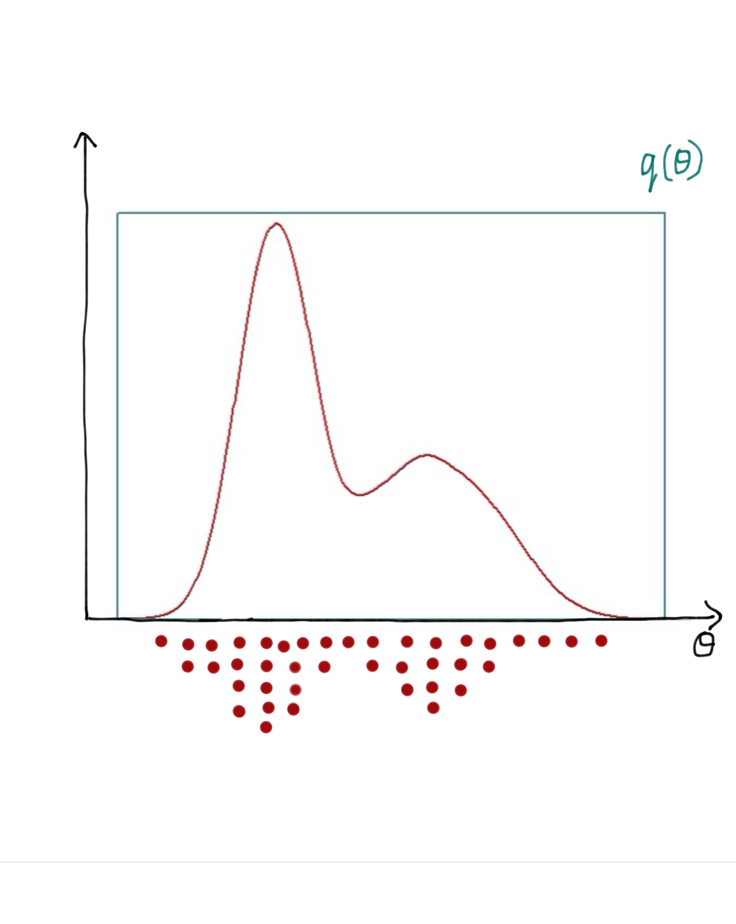
\includegraphics[width=1\linewidth]{RS22.png}}}

    \column{.6\textwidth}
    The algorithm proceeds as follows:\\
    \begin{enumerate}
        \item Sample $\theta^*$ from $q(\theta)$ \\~\\
        \item Draw $u \sim Uniform[0, Mq(\theta^*)]$ \\~\\
        \item Evaluate $f(\theta^*)$ \\~\\
        \item If $f(\theta^*) > u$ accept, else reject \\~\\
        \item Repeat steps 1-4
    \end{enumerate}
\end{columns}
\end{frame}

\begin{frame}[label=sec-5-9]{Rejection sampling}
    \begin{columns}[c] 
    \column{.6\textwidth}
    \begin{itemize}
        \item Rejection sampling works best if $q(\theta) \approx f(\theta)$ ($M\gtrapprox 1$)\\~\\
        \item Acceptance rate of rejection sampler is $\frac{1}{M}$\\~\\
        \item Requiring $f(\theta) < Mq(\theta)$ for all $\theta$ can make rejection rate v. high\\~\\
        \item Even more limited in high dimensions
    \end{itemize}

    \column{.5\textwidth}
    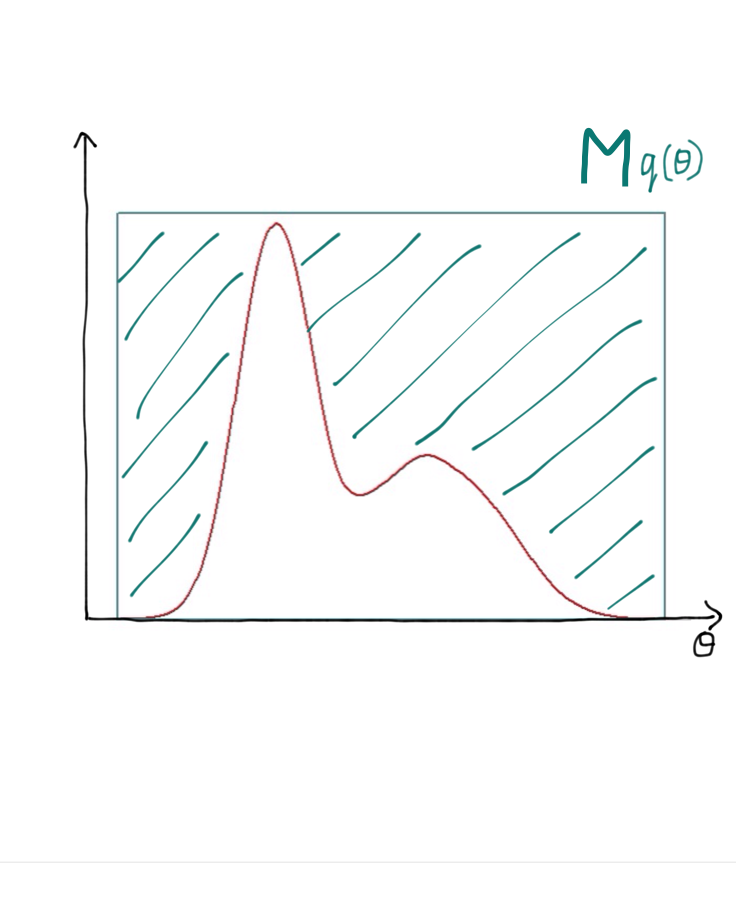
\includegraphics[width=1\linewidth]{RS23.png}
\end{columns}
\end{frame}


\section{What is Markov Chain Monte Carlo?}
\label{sec-7}
\begin{frame}[label=sec-7-1]{Markov Chain Monte Carlo}
    \begin{itemize}
        \item In Markov Chain Monte Carlo (MCMC) we do not define one proposal density $q(\theta)$ such that $ f(\theta) < M q(\theta)$.\\~\\
        \item Rather we build up a \alert{chain} of samples where each proposed $\theta^*$ depends on the previous one \\~\\
        i.e the proposal density takes the form $q(\theta^* | \theta)$\\~\\
        \item A commonly used MCMC algorithm is \alert{Metropolis-Hastings} (M-H).\\~\\
        \item The acceptance rate of M-H is carefully derived to ensure \alert{unbiased samples}.
    \end{itemize}
\end{frame}


\begin{frame}[label=sec-7-2]{Metropolis-Hastings}
    \begin{columns}[c] 
    \column{.5\textwidth} 
    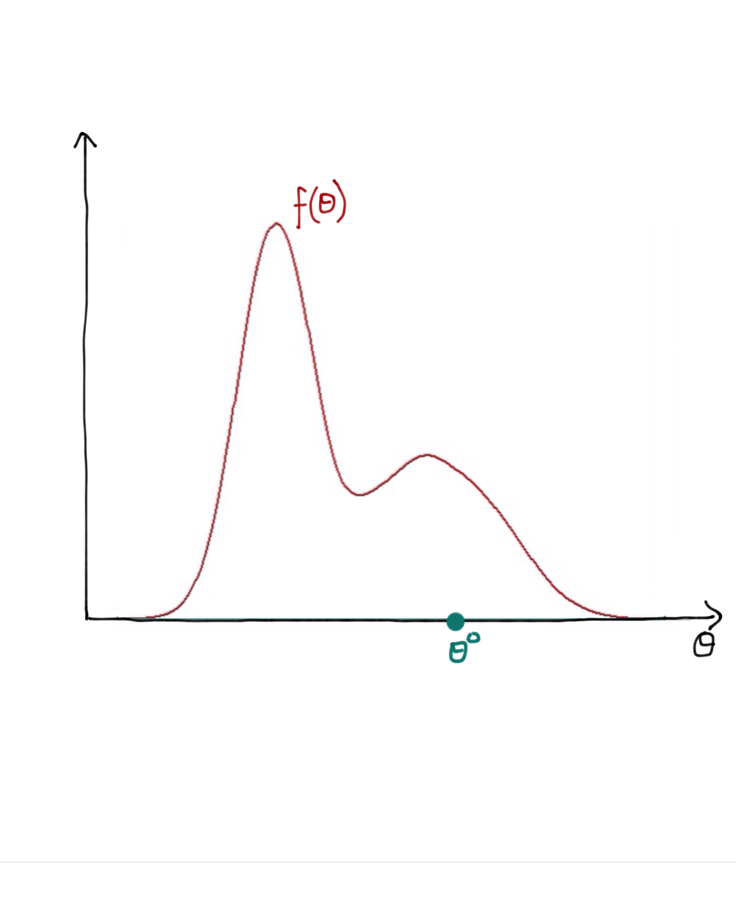
\includegraphics[width=1\linewidth]{MH1}

    \column{.6\textwidth}
    The algorithm proceeds as follows:\\
    \begin{enumerate}
        \item Initialise $\theta^{0}$, set $\theta = \theta^{0}$
        \textcolor{white}{
            \item[\color{white}] Sample $\theta^* \sim q(\theta^*|\theta)$
            \item[\color{white}] Compute acceptance probability, r
            \item[\color{white}] Draw $u \sim Uniform[0,1]$
            \item[\color{white}] Set new sample to 
            \[
               \theta^{(s+1)} = 
               \begin{cases}
                \theta^*, & \text{if } u < r\\
                \theta^{(s)}, & \text{if } u \geqslant r
            \end{cases}
        \]
        \item[\color{white}] Repeat steps 2-5
    }
\end{enumerate}
\end{columns}
\end{frame}


\begin{frame}[label=sec-7-3]{Metropolis-Hastings}
    \begin{columns}[c] 
    \column{.5\textwidth} 
    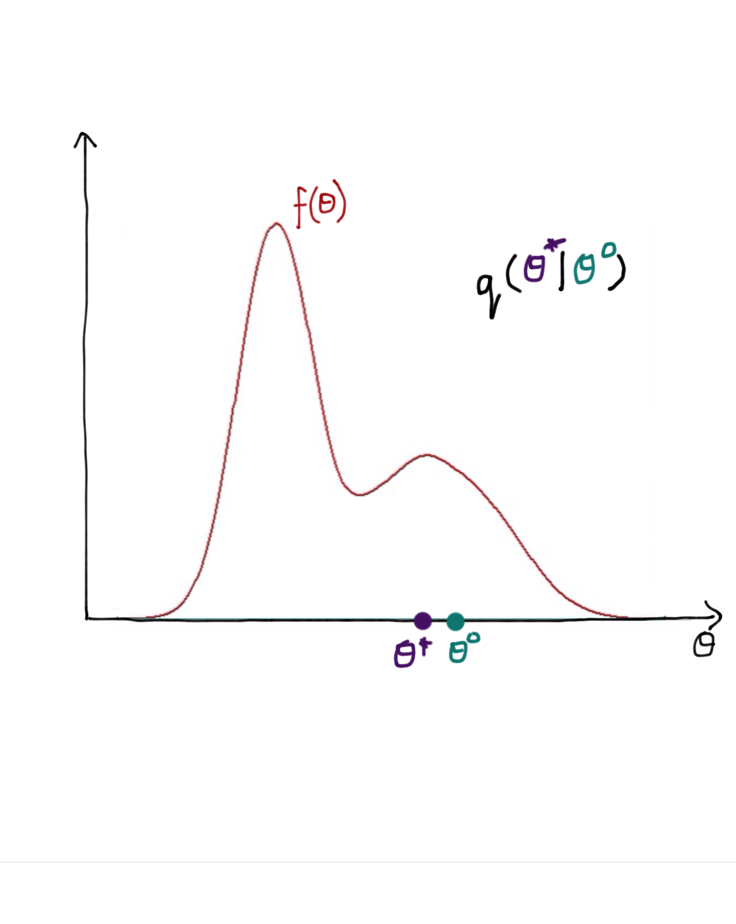
\includegraphics[width=1\linewidth]{MH2}

    \column{.6\textwidth}
    The algorithm proceeds as follows:
    \begin{enumerate}
        \item Initialise $\theta^{0}$, set $\theta = \theta^{0}$
        \item Sample $\theta^* \sim q(\theta^*|\theta)$
        \textcolor{white}{
            \item[\color{white}] Compute acceptance probability, r
            \item[\color{white}] Draw $u \sim Uniform[0,1]$
            \item[\color{white}] Set new sample to 
            \[
               \theta^{(s+1)} = 
               \begin{cases}
                \theta^*, & \text{if } u < r\\
                \theta^{(s)}, & \text{if } u \geqslant r
            \end{cases}
        \]
        \item[\color{white}] Repeat steps 2-5
    }
\end{enumerate}
\end{columns}
\end{frame}


\begin{frame}[label=sec-7-4]{Metropolis-Hastings}
    \begin{columns}[c] 
    \column{.5\textwidth} 
    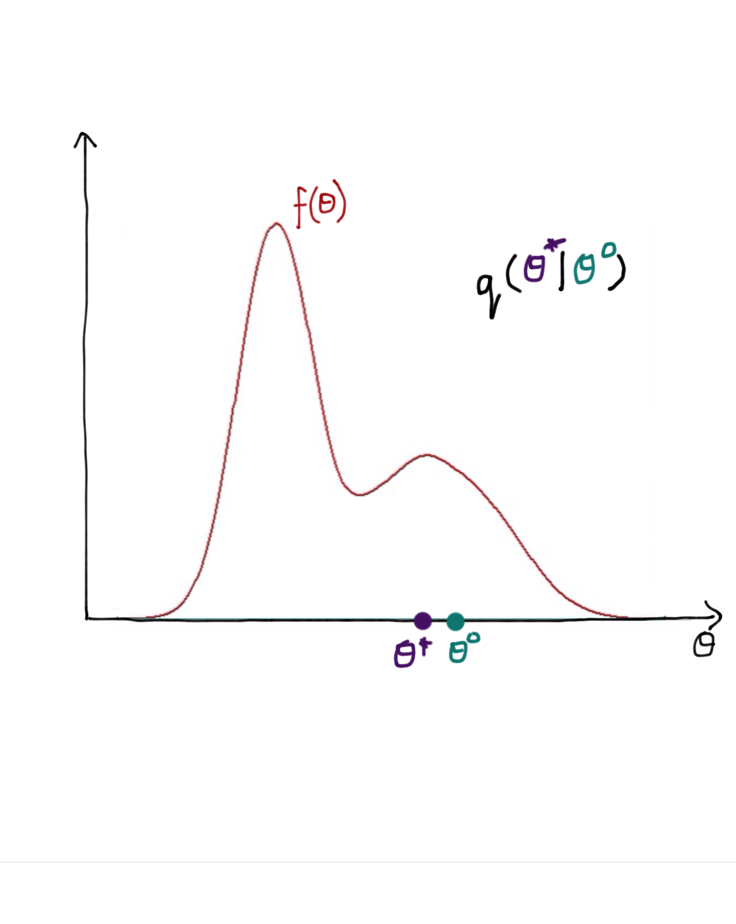
\includegraphics[width=1\linewidth]{MH2}

    \column{.6\textwidth}
    The algorithm proceeds as follows:\\
    \begin{enumerate}
        \item Initialise $\theta^{0}$, set $\theta = \theta^{0}$
        \item Sample $\theta^* \sim q(\theta^*|\theta)$
        \item Compute acceptance probability, r
        \textcolor{white}{
            \item[\color{white}] Draw $u \sim Uniform[0,1]$
            \item[\color{white}] Set new sample to 
            \[
               \theta^{(s+1)} = 
               \begin{cases}
                \theta^*, & \text{if } u < r\\
                \theta^{(s)}, & \text{if } u \geqslant r
            \end{cases}
        \]
        \item[\color{white}] Repeat steps 2-5
    }
\end{enumerate}
\end{columns}
\end{frame}

\begin{frame}[label=sec-7-5]{Metropolis-Hastings}
    \begin{columns}[c] 
    \column{.5\textwidth} 
    \begin{block}{Acceptance}
        \begin{itemize}
            \item If $q(\theta^*|\theta)$ symmetric, then 
            $$ r = min \left( 1,\dfrac{f(\theta^*)}{f(\theta)} \right)$$ 
            \textcolor{white}{
                \item[\color{white}] Definitely move to $\theta^*$ if more probable than $\theta$ 
                \item[\color{white}] May move if $\theta^*$ less probable \\~\\
                \item[\color{white}] If $q(\theta^*|\theta)$ asymmetric, then $$ r = min \left( 1,\dfrac{f(\theta^*)q(\theta|\theta^*)}{f(\theta)q(\theta^*|\theta)} \right)$$
            }
        \end{itemize}
    \end{block}

    \column{.6\textwidth}
    The algorithm proceeds as follows:\\
    \begin{enumerate}
        \item Initialise $\theta^{0}$, set $\theta = \theta^{0}$
        \item Sample $\theta^* \sim q(\theta^*|\theta)$
        \item Compute acceptance probability, r
        \textcolor{white}{
            \item[\color{white}] Draw $u \sim Uniform[0,1]$
            \item[\color{white}] Set new sample to 
            \[
               \theta^{(s+1)} = 
               \begin{cases}
                \theta^*, & \text{if } u < r\\
                \theta^{(s)}, & \text{if } u \geqslant r
            \end{cases}
        \]
        \item[\color{white}] Repeat steps 2-5
    }
\end{enumerate}
\end{columns}
\end{frame}

\begin{frame}[label=sec-7-6]{Metropolis-Hastings}
    \begin{columns}[c] 
    \column{.5\textwidth} 
    \begin{block}{Acceptance}
        \begin{itemize}
            \item If $q(\theta^*|\theta)$ symmetric, then 
            $$ r = min \left( 1,\dfrac{f(\theta^*)}{f(\theta)} \right)$$ 
            \item Definitely move to $\theta^*$ if more probable than $\theta$ 
            \textcolor{white}{
                \item[\color{white}] May move if $\theta^*$ less probable \\~\\
                \item[\color{white}] If $q(\theta^*|\theta)$ asymmetric, then $$ r = min \left( 1,\dfrac{f(\theta^*)q(\theta|\theta^*)}{f(\theta)q(\theta^*|\theta)} \right)$$
            }
        \end{itemize}
    \end{block}

    \column{.5\textwidth}
    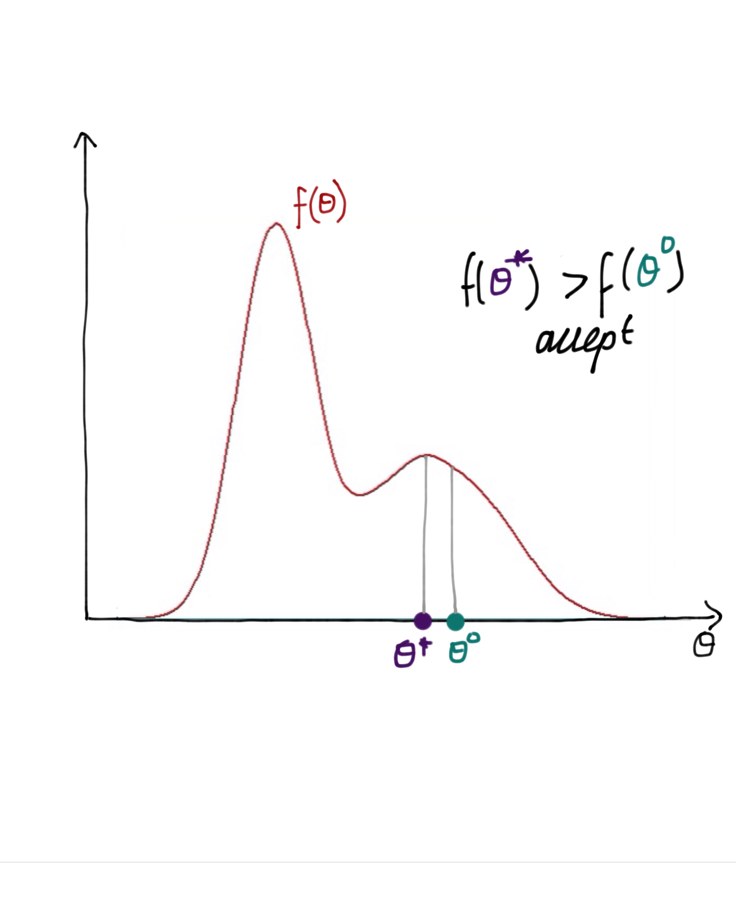
\includegraphics[width=1\linewidth]{MH3}
\end{columns}
\end{frame}

\begin{frame}[label=sec-7-7]{Metropolis-Hastings}
    \begin{columns}[c] 
    \column{.5\textwidth} 
    \begin{block}{Acceptance}
        \begin{itemize}
            \item If $q(\theta^*|\theta)$ symmetric, then 
            $$ r = min \left( 1,\dfrac{f(\theta^*)}{f(\theta)} \right)$$ 
            \item Definitely move to $\theta^*$ if more probable than $\theta$ 
            \item May move if $\theta^*$ less probable \\~\\
            \textcolor{white}{
                \item[\color{white}] If $q(\theta^*|\theta)$ asymmetric, then $$ r = min \left( 1,\dfrac{f(\theta^*)q(\theta|\theta^*)}{f(\theta)q(\theta^*|\theta)} \right)$$
            }
        \end{itemize}
    \end{block}

    \column{.5\textwidth}
    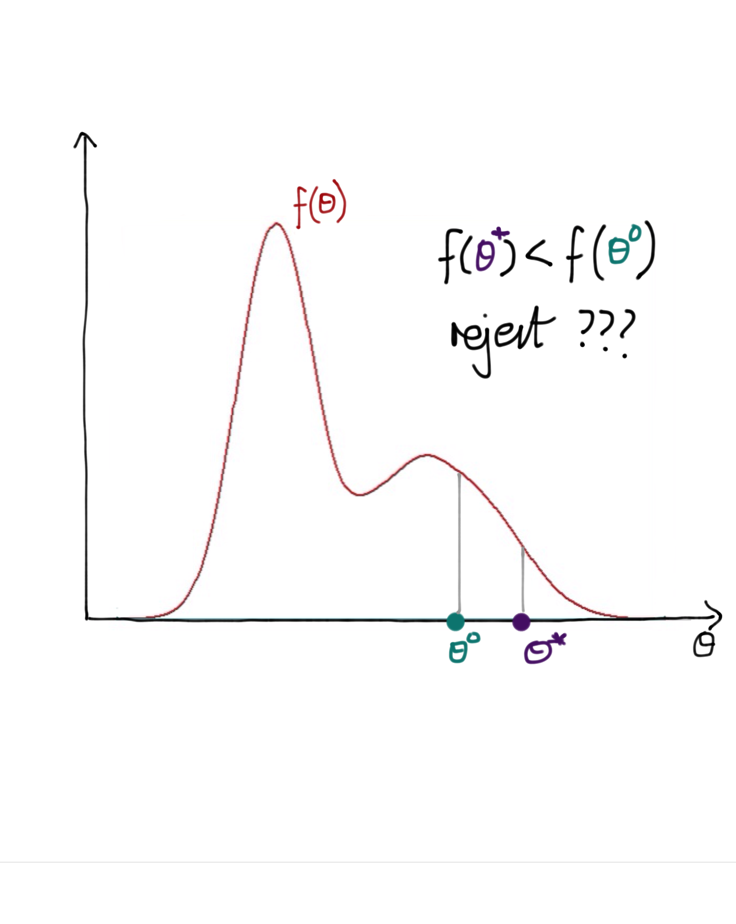
\includegraphics[width=1\linewidth]{MH4}
\end{columns}
\end{frame}

\begin{frame}[label=sec-7-8]{Metropolis-Hastings}
    \begin{columns}[c] 
    \column{.5\textwidth} 
    \begin{block}{Acceptance}
        \begin{itemize}
            \item If $q(\theta^*|\theta)$ symmetric, then 
            $$ r = min \left( 1,\dfrac{f(\theta^*)}{f(\theta)} \right)$$ 
            \item Definitely move to $\theta^*$ if more probable than $\theta$ 
            \item May move if $\theta^*$ less probable \\~\\
            \item If $q(\theta^*|\theta)$ asymmetric, then $$ r = min \left( 1,\dfrac{f(\theta^*)q(\theta|\theta^*)}{f(\theta)q(\theta^*|\theta)} \right)$$
        \end{itemize}
    \end{block}

    \column{.5\textwidth}
    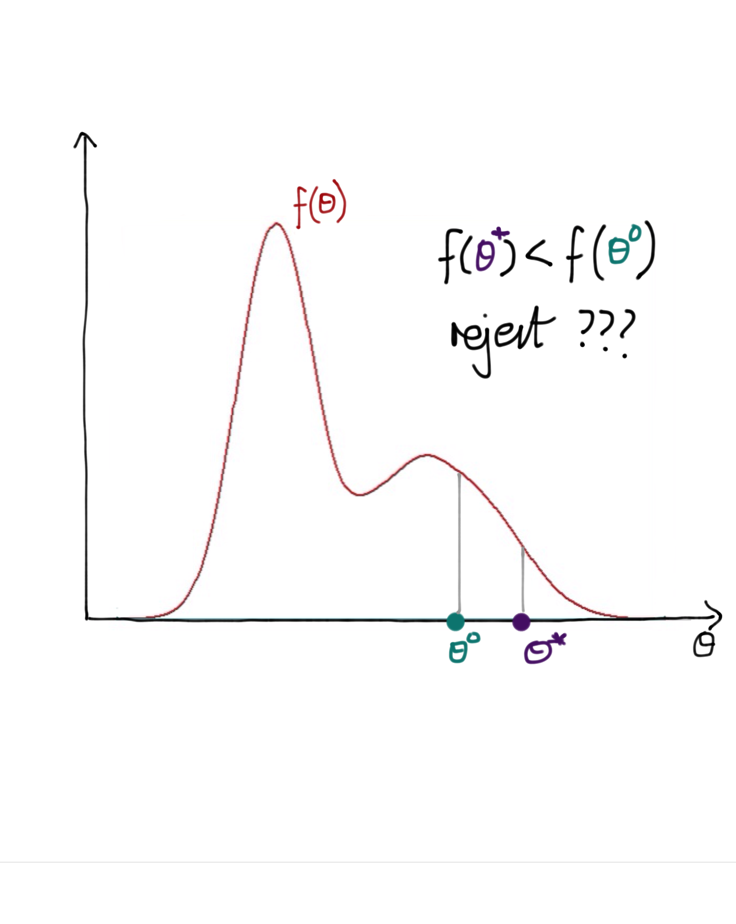
\includegraphics[width=1\linewidth]{MH4}
\end{columns}
\end{frame}

\begin{frame}[label=sec-7-9]{Metropolis-Hastings}
    \begin{columns}[c] 
    \column{.5\textwidth} 
    \begin{block}{Acceptance}
        \begin{itemize}
            \item If $q(\theta^*|\theta)$ symmetric, then 
            $$ r = min \left( 1,\dfrac{f(\theta^*)}{f(\theta)} \right)$$ 
            \item Definitely move to $\theta^*$ if more probable than $\theta$ 
            \item May move if $\theta^*$ less probable \\~\\
            \item If $q(\theta^*|\theta)$ asymmetric, then $$ r = min \left( 1,\dfrac{f(\theta^*)q(\theta|\theta^*)}{f(\theta)q(\theta^*|\theta)} \right)$$
        \end{itemize}
    \end{block}

    \column{.6\textwidth}
    The algorithm proceeds as follows:\\
    \begin{enumerate}
        \item Initialise $\theta^{0}$, set $\theta = \theta^{0}$
        \item Sample $\theta^* \sim q(\theta^*|\theta)$
        \item Compute acceptance probability, r
        \textcolor{white}{
            \item[\color{white}] Draw $u \sim Uniform[0,1]$
            \item[\color{white}] Set new sample to 
            \[
               \theta^{(s+1)} = 
               \begin{cases}
                \theta^*, & \text{if } u < r\\
                \theta^{(s)}, & \text{if } u \geqslant r
            \end{cases}
        \]
        \item[\color{white}] Repeat steps 2-5
    }
\end{enumerate}
\end{columns}
\end{frame}

\begin{frame}[label=sec-7-10]{Metropolis-Hastings}
    \begin{columns}[c] 
    \column{.5\textwidth} 
    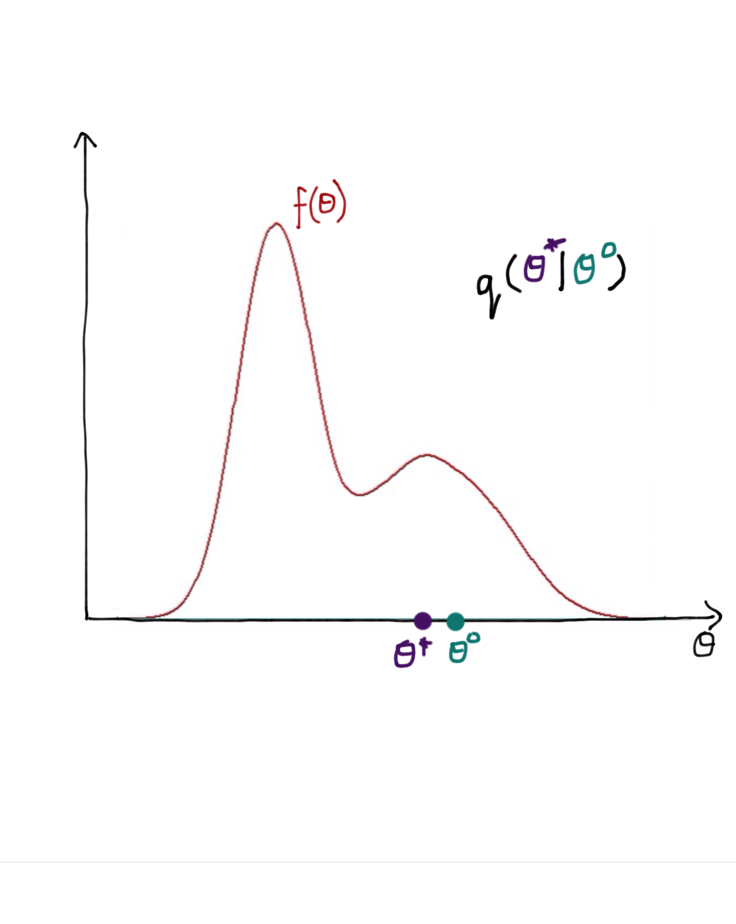
\includegraphics[width=1\linewidth]{MH2}

    \column{.6\textwidth}
    The algorithm proceeds as follows:\\
    \begin{enumerate}
        \item Initialise $\theta^{0}$, set $\theta = \theta^{0}$
        \item Sample $\theta^* \sim q(\theta^*|\theta)$
        \item Compute acceptance probability, r
        \textcolor{white}{
            \item[\color{white}] Draw $u \sim Uniform[0,1]$
            \item[\color{white}] Set new sample to 
            \[
               \theta^{(s+1)} = 
               \begin{cases}
                \theta^*, & \text{if } u < r\\
                \theta^{(s)}, & \text{if } u \geqslant r
            \end{cases}
        \]
        \item[\color{white}] Repeat steps 2-5
    }
\end{enumerate}
\end{columns}
\end{frame}

\begin{frame}[label=sec-7-11]{Metropolis-Hastings}
    \begin{columns}[c] 
    \column{.5\textwidth} 
    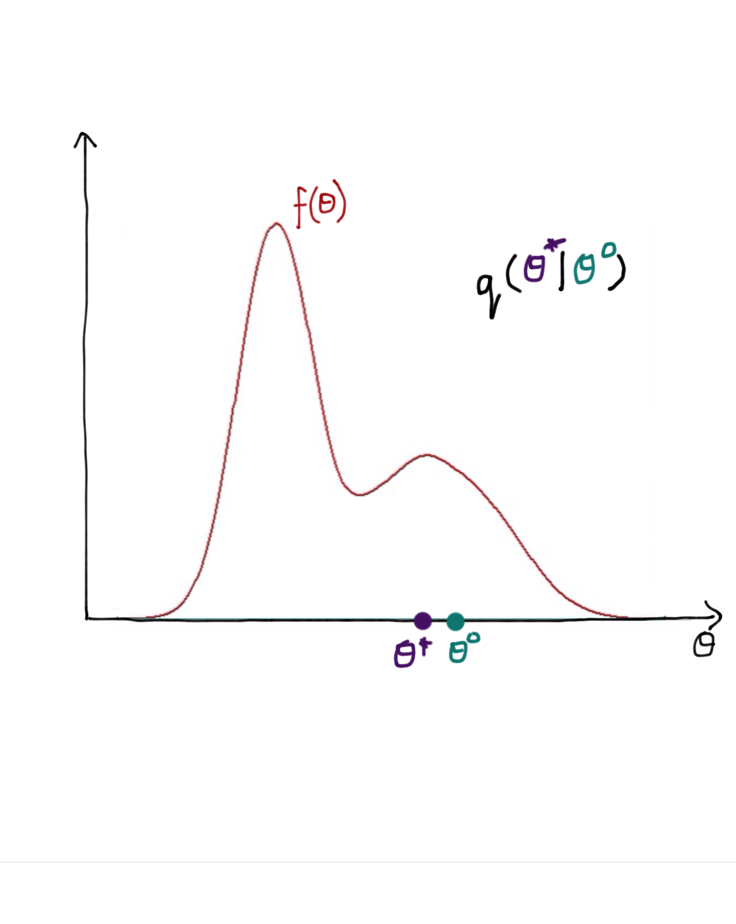
\includegraphics[width=1\linewidth]{MH2}

    \column{.6\textwidth}
    The algorithm proceeds as follows:\\
    \begin{enumerate}
        \item Initialise $\theta^{0}$, set $\theta = \theta^{0}$
        \item Sample $\theta^* \sim q(\theta^*|\theta)$
        \item Compute acceptance probability, r
        \item Draw $u \sim Uniform[0,1]$
        \textcolor{white}{
            \item[\color{white}] Set new sample to 
            \[
               \theta^{(s+1)} = 
               \begin{cases}
                \theta^*, & \text{if } u < r\\
                \theta^{(s)}, & \text{if } u \geqslant r
            \end{cases}
        \]
        \item[\color{white}] Repeat steps 2-5
    }
\end{enumerate}
\end{columns}
\end{frame}

\begin{frame}[label=sec-7-12]{Metropolis-Hastings}
    \begin{columns}[c] 
    \column{.5\textwidth} 
    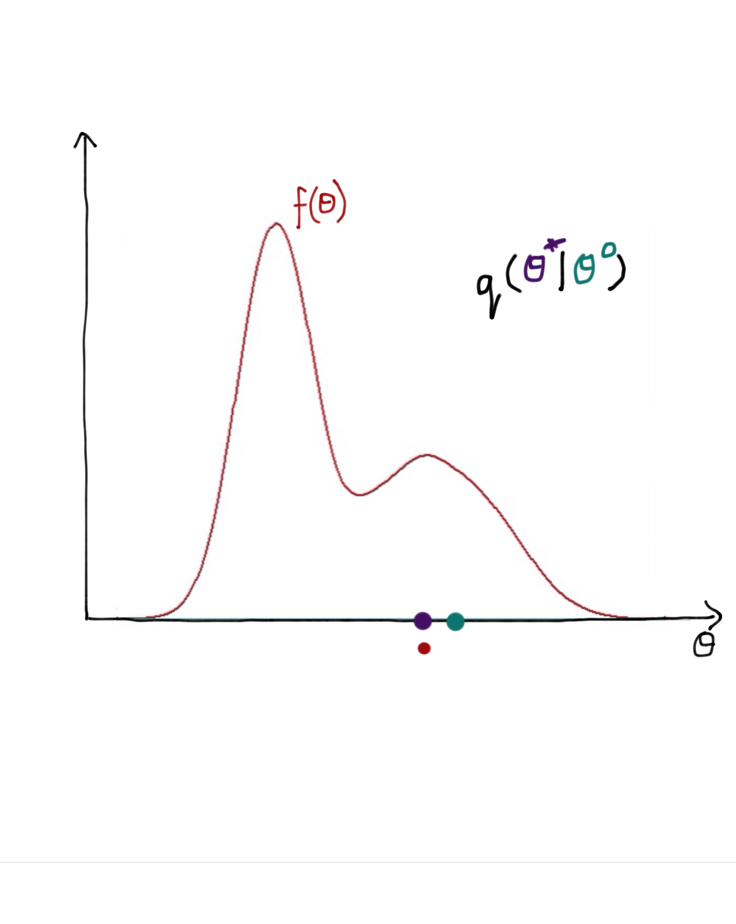
\includegraphics[width=1\linewidth]{MH5}

    \column{.6\textwidth}
    The algorithm proceeds as follows:\\
    \begin{enumerate}
        \item Initialise $\theta^{0}$, set $\theta = \theta^{0}$
        \item Sample $\theta^* \sim q(\theta^*|\theta)$
        \item Compute acceptance probability, r
        \item Draw $u \sim Uniform[0,1]$
        \item Set new sample to 
        \[
           \theta^{(s+1)} = 
           \begin{cases}
            \theta^*, & \text{if } u < r\\
            \theta^{(s)}, & \text{if } u \geqslant r
        \end{cases}
    \]
    \textcolor{white}{
        \item[\color{white}] Repeat steps 2-5
    }
\end{enumerate}
\end{columns}
\end{frame}

\begin{frame}[label=sec-7-13]{Metropolis-Hastings}
    \begin{columns}[c] 
    \column{.5\textwidth} 
    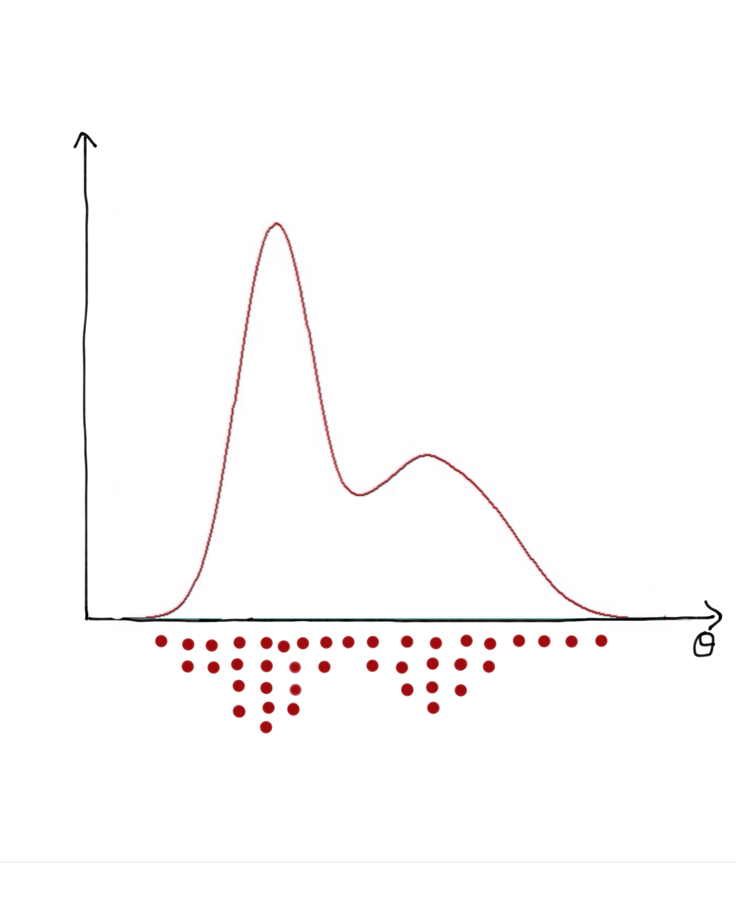
\includegraphics[width=1\linewidth]{MH6}

    \column{.6\textwidth}
    The algorithm proceeds as follows:\\
    \begin{enumerate}
        \item Initialise $\theta^{0}$, set $\theta = \theta^{0}$
        \item Sample $\theta^* \sim q(\theta^*|\theta)$
        \item Compute acceptance probability, r
        \item Draw $u \sim Uniform[0,1]$
        \item Set new sample to 
        \[
           \theta^{(s+1)} = 
           \begin{cases}
            \theta^*, & \text{if } u < r\\
            \theta^{(s)}, & \text{if } u \geqslant r
        \end{cases}
    \]
    \item Repeat steps 2-5
\end{enumerate}
\end{columns}
\end{frame}

\section{MCMC in practice}
\label{sec-8}
\begin{frame}[label=sec-8-1]{Review}
    In the practical you used \textit{Metropolis-Hastings} with a \textit{Gaussian} proposal distribution to infer \textit{one} parameter, $R_0$\\~\\

    In this session we will:
    \begin{itemize}
        \item extend to multivariate inference
        \item learn about MCMC diagnostics
        \item think about accuracy and efficiency
    \end{itemize}
\end{frame}

\begin{frame}[label=sec-8-2]{Interlude: Multivariate Gaussian distribution}
    To infer more multiple parameters we can use multivariate Gaussian\\~\\
    \begin{columns}[c] 
    \column{.5\textwidth} 
    mean $\mu = \begin{bmatrix} 3 & 2 \end{bmatrix}$\\
    covariance $\Sigma =  \begin{bmatrix} 25 & 0 \\ 0 & 9 \end{bmatrix}$
    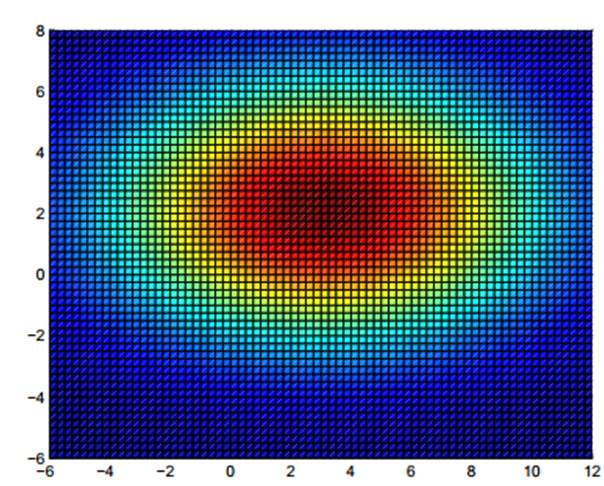
\includegraphics[width=0.8\linewidth]{MVN1}

    \column{.5\textwidth}
    mean $\mu = \begin{bmatrix} 3 & 2 \end{bmatrix}$\\
    covariance $\Sigma =  \begin{bmatrix} 10 & 5 \\ 5 & 5 \end{bmatrix}$
    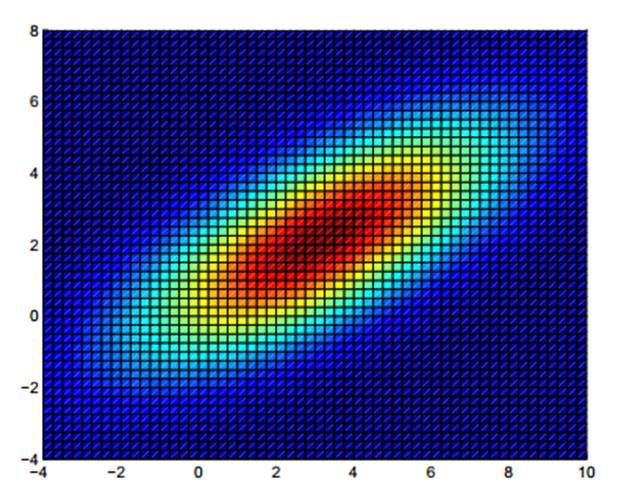
\includegraphics[width=0.8\linewidth]{MVN2}
\end{columns}  
For accurate and efficient MCMC we tune the variance and covariance of the proposal distribution.
\end{frame}

\begin{frame}[label=sec-8-3]{Choosing a proposal distribution}
    If \alert {variance is too small}, the chain will be slow to reach the target distribution.
    \begin{columns}[c] 
    \column{.5\textwidth} 
    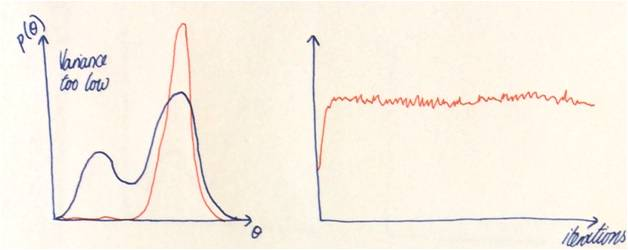
\includegraphics[width=0.8\linewidth]{Var1}
    \column{.5\textwidth}
    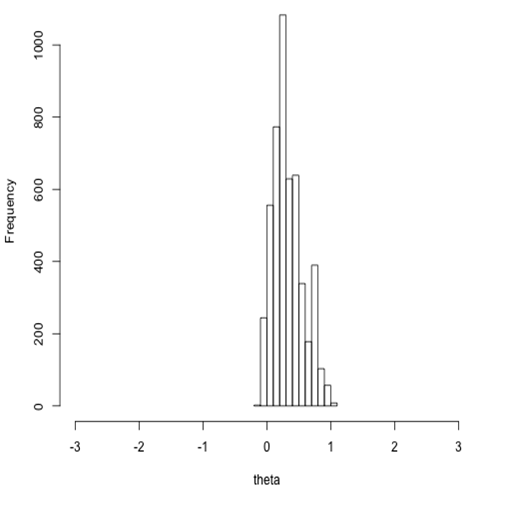
\includegraphics[width=0.8\linewidth]{Trace1}
\end{columns}  
\end{frame}

\begin{frame}[label=sec-8-4]{Choosing a proposal distribution}
    If \alert{variance is too high}, many proposed values will be rejected and the chain will \textit{stick} in one place for many steps.
    \begin{columns}[c] 
    \column{.5\textwidth} 
    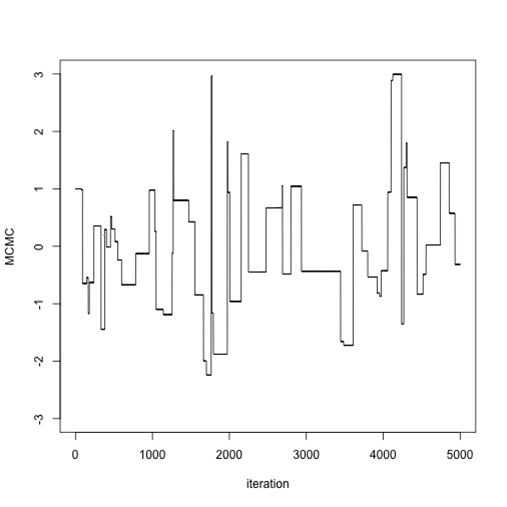
\includegraphics[width=0.8\linewidth]{Var2}
    \column{.5\textwidth}
    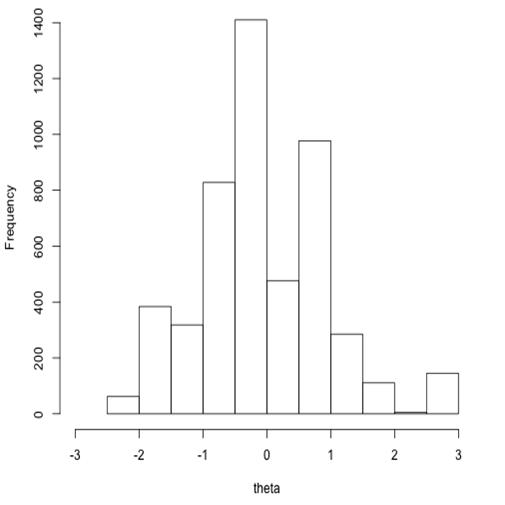
\includegraphics[width=0.8\linewidth]{Trace2}
\end{columns}  
\end{frame}

\begin{frame}[label=sec-8-5]{Choosing a proposal distribution}
    If \alert{variance is just right}, the chain will efficiently explore the full shape of the target distribution.
    \begin{columns}[c] 
    \column{.5\textwidth} 
    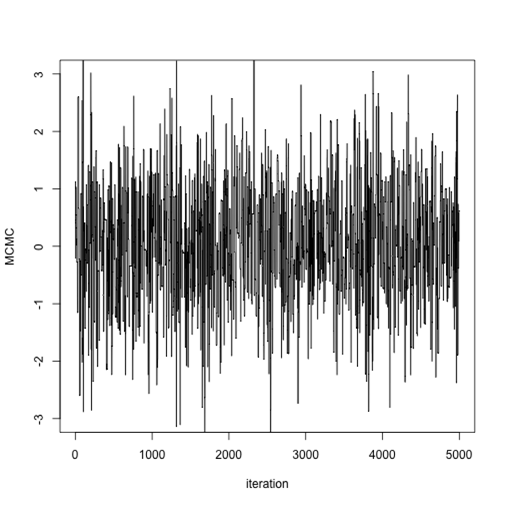
\includegraphics[width=0.8\linewidth]{Var3}
    \column{.5\textwidth}
    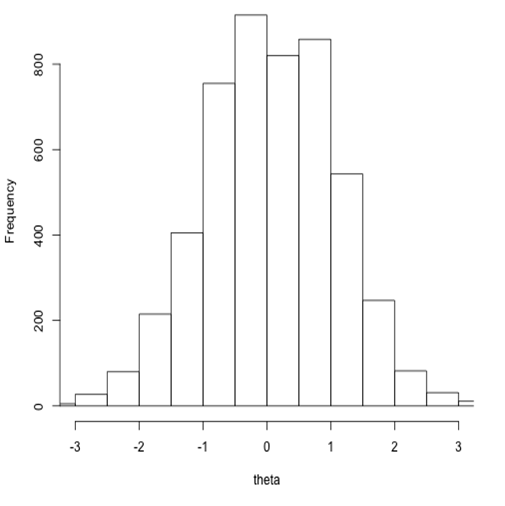
\includegraphics[width=0.8\linewidth]{Trace3}
\end{columns}  
Try several different proposal distributions (\alert{pilot runs}), aiming for an acceptance rate between 24\%  and 40\%. 
\end{frame}

\begin{frame}[label=sec-8-6]{Adaptive MCMC}
    \begin{itemize}
        \item \alert{Adaptive MCMC} alters proposal distribution while chain is running. \\~\\
        \item Start with large symmetric variance, scan around to find a mode. \\~\\
        \item Then alter shape of proposal distribution to match covariance matrix of accepted values.\\~\\
        \item Eventually proposal density should match the shape of target density.\\~\\
    \end{itemize}
\end{frame}

\begin{frame}[label=sec-8-7]{Adaptive MCMC}
    Two-stage adaptation
    \begin{columns}[c] 
    \column{.5\textwidth} 
    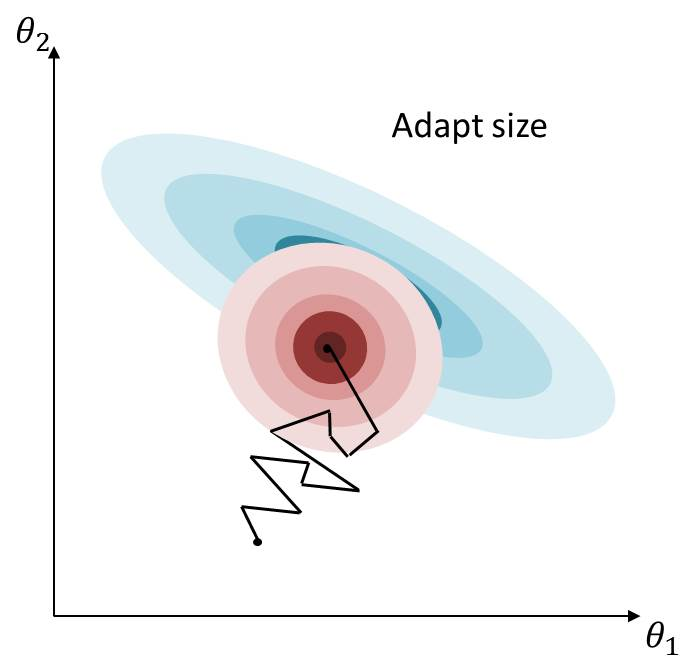
\includegraphics[width=.8\linewidth]{MH7.jpg}
    \column{.5\textwidth} 
    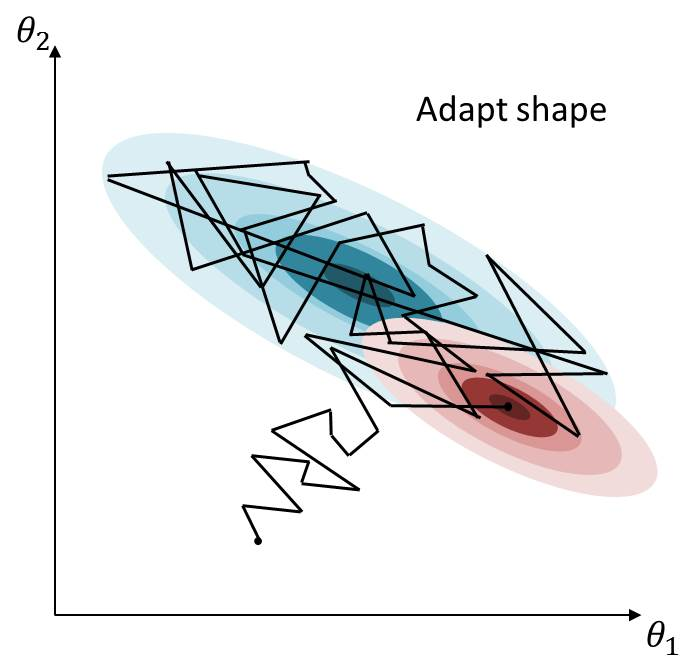
\includegraphics[width=.8\linewidth]{MH8.jpg}
\end{columns}
\end{frame}

\begin{frame}[label=sec-8-8]{Burn-in}
    \begin{columns}[c] 
    \column{.6\textwidth} 
    \begin{itemize}
        \item We can start our MCMC chain anywhere. \\~\\
        \item It can take a while to reach and explore the target density $f(\theta)$. \\~\\
        \item Throw away early samples: \alert{burn-in} phase. \\~\\
        \item How much to discard? \\~\\
    \end{itemize}
    \column{.5\textwidth} 
    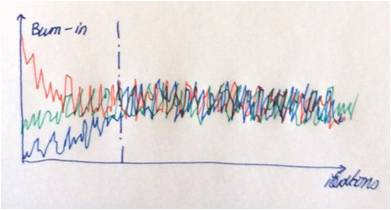
\includegraphics[width=1\linewidth]{Burn}
\end{columns}
\end{frame} 

\begin{frame}[label=sec-8-9]{MCMC sample size}
    \begin{itemize}
        \item In MCMC, each sample depends on the one before - \alert{auto-correlation} \\~\\
        \item Reduce degree of auto-correlation by \alert{thinning}, only retain every $n^{th}$ sample. \\~\\
        \item Information content of MCMC samples is given by the \alert{effective sample size (ESS)}. \\~\\
        \item We use the R package \textit{coda}.
    \end{itemize}
\end{frame}

\end{document}
